
\chapter{Background}\label{chapter:background}

\section{RDF}

\section{Foundations of Statistics} \label{section:distributions}
In this section, we present the fundamental concepts of the field of statistics. The majority of the definitions can be found in~\cite{statistics_book}.

\subsection{Population and Sample}

A \textbf{population} is a large set of objects of a similar nature, and the \textbf{sample} is a subset of objects derived from a population~\cite{sample1}. A population includes all of the elements from a set of data, however, a sample consists of one or more observations from the population~\cite{sample2}.\\
The sample size is the number of observations in a sample and commonly denoted by \textit{n}.

\subsection{Probability Distributions}

The probability distribution links each possible value of a random variable~\cite{random_variable} with its probability of occurrence. The following paragraphs we define different discrete probability distributions related to our work.

\subsubsection{Uniform Distribution}

A random variable $X$ has a discrete uniform distribution if each of the \textit{n} values in
its range, namely, $x_1$, $x_2$, ..., $x_n$, has equal probability. Formally:
\begin{align}
	f(x_i) = \frac{1}{n}
\end{align}
where $f(x_i)$ denotes the probability distribution function.

\subsubsection{Power-Law Distribution}

%If $X$ is a random variable with a Pareto distribution\footnote{More types of Pareto distributions are distinguished, the commonly known Type I %distribution is introduced.}, then the probability that $X$ is greater than some number $\sigma$, is given by
%\begin{align}
%	\overline{F}(x) = Pr(X>\sigma) = \Big( \frac{x}{\sigma} \Big)^{-\alpha}
%\end{align}
%where $\sigma$ is the scale, and $\alpha$ represents the shape parameter($x$ > $\sigma$, $\sigma$ > 0).

The power-law distribution describes the probability of the random variable that is equal to $x$ as the following
\begin{align}
	f(x) = c\cdot x^{-\gamma}
\end{align}
where $c$ is a constant and $\gamma$ is called as the \textit{exponent} or \textit{scale factor}.

\subsubsection{Poisson Distribution}
The Poisson distribution is characterized by the following elementary probabilities:
\begin{align}
	P(X = k) = \frac{\lambda^k}{k!}e^{-\lambda}
\end{align}
where $\lambda$ > 0 is the shape parameter and $k$ $\in$ $\mathbb{N}$.

%todo insert distributions pic%

\subsection{Related Measurements}

\subsubsection{Mean}
The \textit{mean} or \textit{expected value} of a discrete random variable $X$ denoted by $\mu$ or $E(X)$ is
\begin{align}
	\mu = E(X) = \sum_{x} xf(x)
\end{align}
where $x$ represents the values of the random variable $X$, and $f(x)$ denotes the probability distribution function. A mean is a measure of the center of the probability distribution.

\subsubsection{Variance}

The \textit{variance} of $X$---denoted by $\sigma^2$ or $V(X)$---is equal to the following formula:
\begin{align}
	\sigma^2 = V(X) = E(X - \mu)^2 = \sum_{x}(x - \mu)^2 f(x)
\end{align}

The variance is a measure of the dispersion or variability in the distribution, as it represents the average of the squared differences from the mean. For example, a variance of zero indicates that all the values are identical.

\subsubsection{Standard Deviation}

The \textit{standard deviation} of the random variable $X$ is $\sigma = \sqrt{\sigma^2}$, meaning it is the square root of the variance.

\subsection{Covariance and Correlation}

\subsubsection{Covariance}
The \textit{covariance} is a measure of the linear relationship between random variables. A covariance between two random variables $X$ and $Y$ can be expressed as follows:
\begin{align}
	cov(X,Y) = E\big[(X - \mu_X)(Y - \mu_Y)\big]
\end{align}
A positive covariance implies that $Y$ tends to increase as $X$ increases as well, and if $cov(X,Y) < 0$ then $Y$ tends to decrease as $X$ increases~\cite{covariance}. A few examples of different scenarios are illustrated in Figure \ref{fig:covariance} (~\cite{statistics_book}). In the terms of (a) and (b), a covariance is observable between $X$ and $Y$, and in the cases of (c) and (d), the covariance is equal to zero.

\begin{figure}[!ht]
	\centering
	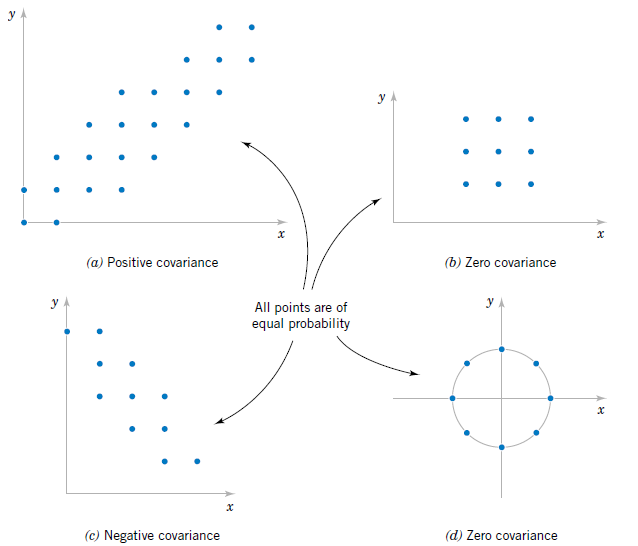
\includegraphics[width=140mm, keepaspectratio]{figures/covariance.png}
	\caption{Different examples for covariance.}
	\label{fig:covariance}
\end{figure}

\subsubsection{Correlation}
Similarly to covariance, the \textit{correlation} describes the strength of the relationship between variables. A type of correlation, the Pearson product-moment correlation coefficient is formulated as
\begin{align}
	\rho_{XY} = \frac{cov(X, Y)}{\sigma_X\sigma_Y}
\end{align}
where $ -1 \leq \rho_{XY} \leq 1$, and 1 indicates a positive linear relationship between $X$ and $Y$, and -1 means negative linearity, finally, 0 is interpreted as a correlation does not appear between the variables.

\subsection{Regression Analysis}

\textit{Regression analysis} is a statistical technique for exploring the relationship between two or more variables. A regression model can be considered as an equation that relates a random variable $Y$ to a function of a variable $x$ and a constant $\beta$. Formally, a regression model is defined as
\begin{align} \label{eq:linear_regression}
	Y = \beta_0 + \beta_1x + \epsilon
\end{align}
where $Y$ is the dependent or response variable, $x$ is referred as the independent variable or predictor, and $\beta_0$, $\beta_1$ are the regression coefficients---the intercept and the slope. Finally, $\epsilon$ symbolizes the random error.

A multiple linear regression model considers $k$ independent variables, and the equation is extended as follows:
\begin{align}
	Y = \beta_0 + \beta_1x_1 + \beta_2x_2 + \dots + \beta_kx_k + \epsilon
\end{align}

\section{Graph Theory}

In the following sections we introduce the most important graph metrics and network topologies on which we concentrate in our work. We assume that the reader is already familiar with the basic concepts of graph theory, including undirected graph, complete graph, adjacent nodes,
node degrees and shortest paths.
%todo fix these metrics 
\subsection{Metrics}

\subsubsection{Degree Distribution}

The spread among the degrees of the nodes is characterized by a distribution function $P(k)$ which shows the probability that a randomly selected node's degree is equal to $k$. $P(k)$ is called as the degree distribution.

\subsubsection{Clustering Coefficient}

The $C_n$ clustering coefficient of an $n$ node is equal to the proportion of connections found among the neighbors of $n$ divided by the maximum number of connections that can be possibly exist between them. Formally written, in undirected graphs the clustering coefficient of $n$ node is $C_n = \frac{2\cdot e_n}{k_n\cdot(k_n-1) }$, where $k_n$ is the number of neighbors of $n$, and $e_n$ is the number of connected pairs between all neighbors of $n$ (~\cite{clustering_formula}). The clustering coefficient is always quantified between 0 and 1.

An example is showed in Figure \ref{fig:clustering}. In this case, the clustering coefficient of \textsf{A} is $C_A = \frac{2}{6}$, since it has three neighbors, so $k_A = 3$, and only one connection occurs among its adjacent nodes---between \textsf{B} and \textsf{C}---indicating that $e_A = 1$.
\begin{figure}[!ht]
	\centering
	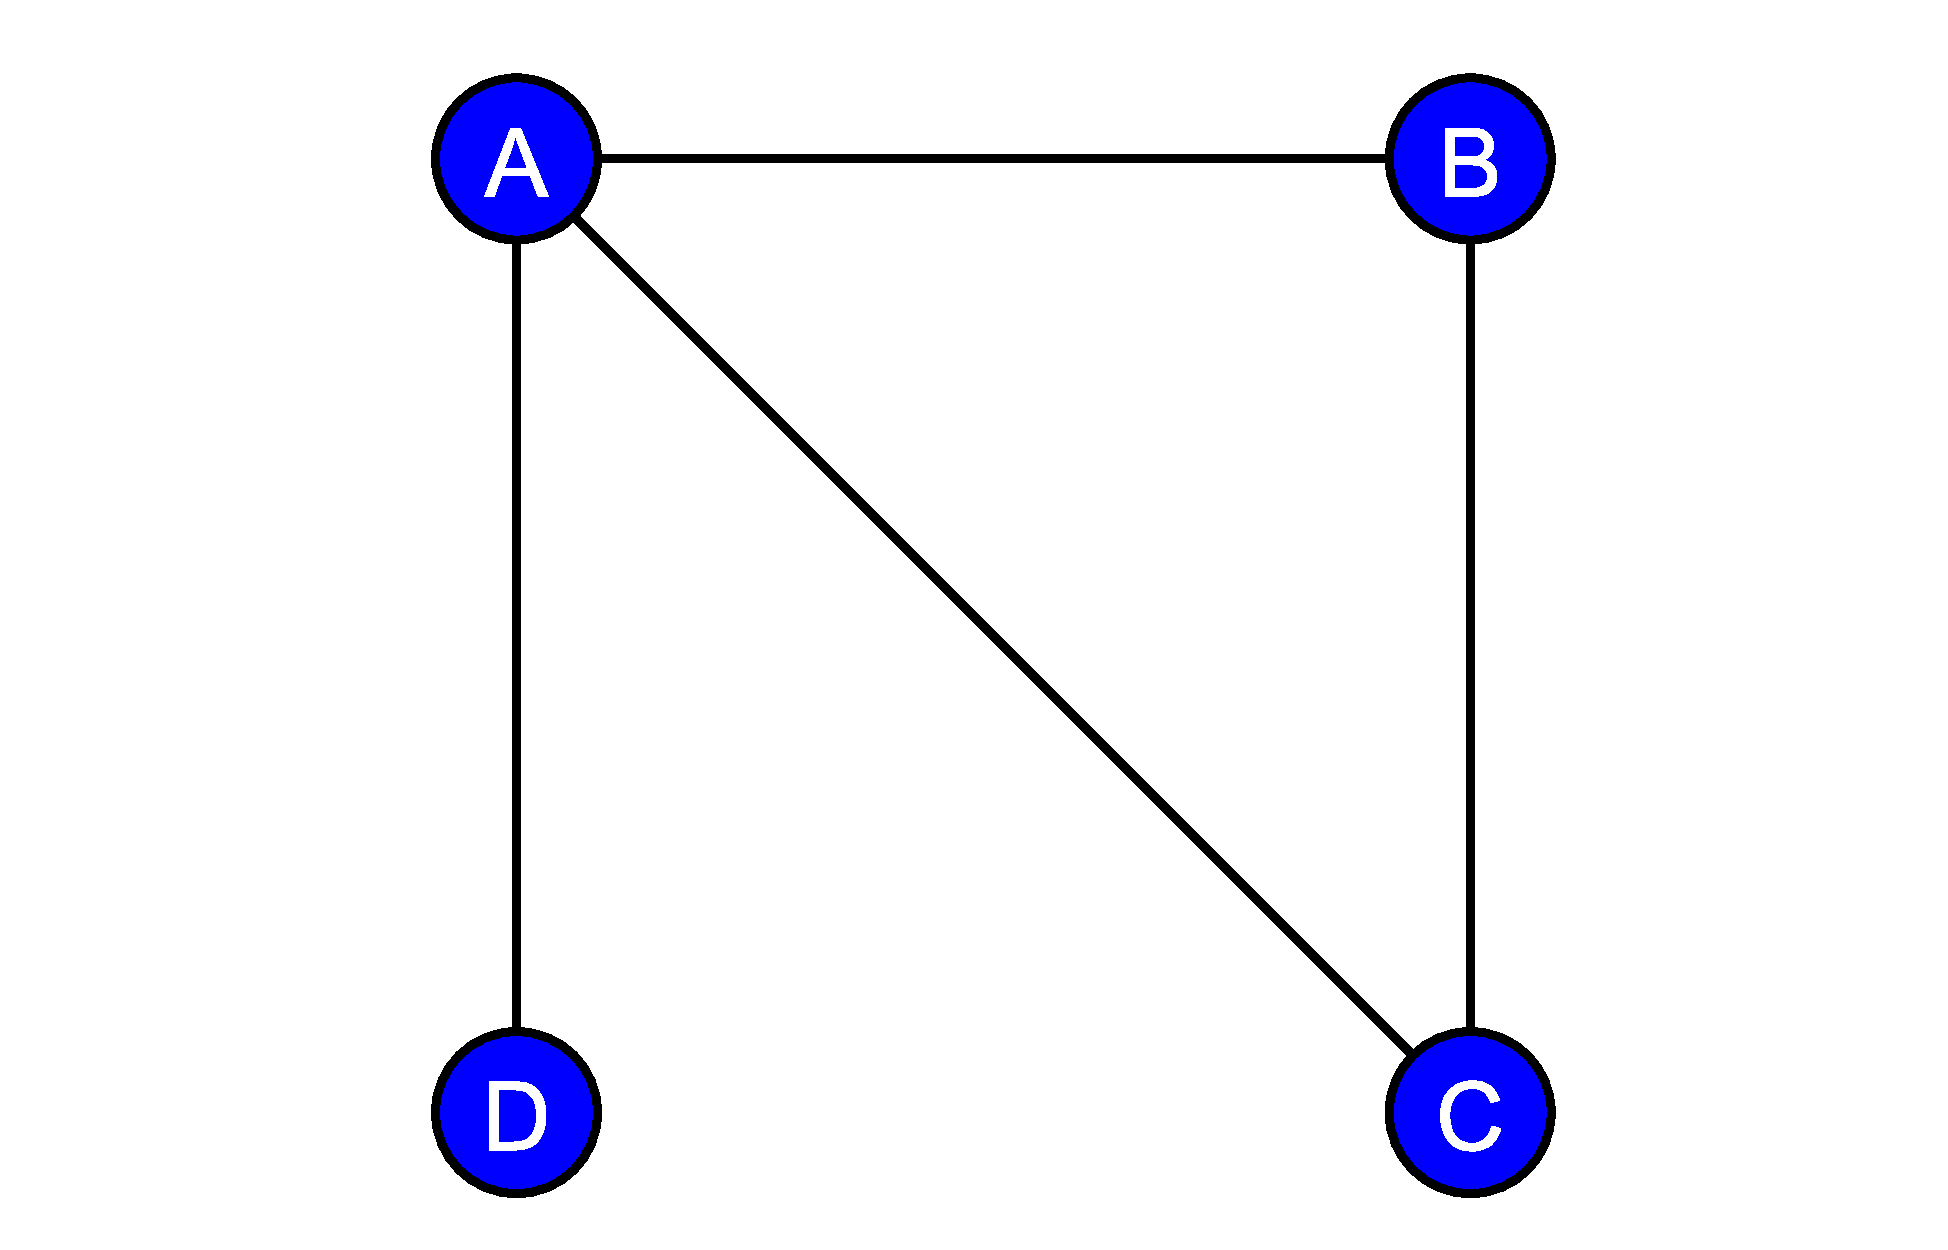
\includegraphics[width=60mm, keepaspectratio]{figures/clustering.pdf}
	\caption{An example graph for illustrating the calculation of the clustering coefficient metric.}
	\label{fig:clustering}
\end{figure}

\subsubsection{Betweenness Centrality}

The betweenness centrality of an $n$ node is quantified by the number of shortest paths that include $n$ as an intermediate node, divided by the entire number of shortest paths. Consequently, this metric is normalized between 0 and 1.

To demonstrate with an example, assume that we searched the following shortest paths denoted by $P_i$:
\begin{itemize}
	\item $P_1 = (v_1, v_3, v_4, v_6, v_5)$
	\item $P_2 = (v_2, v_3, v_4, v_5)$
	\item $P_3 = (v_4, v_3, v_5)$
\end{itemize}

The entire number of shortest paths is equal to three, and the intermediate nodes are $v_3$, $v_4$ and $v_6$. The betweenness centrality values of the nodes---denoted by $B_i$---are the following:
\begin{itemize}
	\item $B_3 = 1$, since $v_3$ appears in all three paths.
	\item $B_4 = \frac{2}{3}$ due to $v_4$ appears in two paths---$P_1$ and $P_2$. Note that $v_4$ in $P_3$ is the initial node and not an intermediate node.
	\item $B_6 = \frac{1}{3}$
	\item $B_1 = B_2 = B_5 = 0$, since they do not appear in the paths as intermediate nodes.
\end{itemize}
\subsection{Network Topologies} \label{sec:topologies}

In the following sections, we introduce the graph topologies that connects to our work. Besides their generation algorithms, we also emphasize the degree distributions they follow.

\subsubsection{Random Graph}

The main concept of the random graph is to create the connections among nodes independently from each other, meaning that the occurrence of an edge between the nodes is not influenced by the other edges. 

Two well-known algorithms exist to create random graphs. The first is the $G(N, M)$ model of Erdős-Rényi~\cite{erdos_random}, and the second is the $G(N,p)$ model from Gilbert~\cite{gilbert_random}. The former means that precisely $M$ number of edges exist among $N$ vertices, and the latter implies that---in the generation algorithm---every pair of nodes becomes adjacent with $p$ probability. The degree distribution of random graphs follows a Poisson distribution.

\subsubsection{Small-World Model of Watts-Strogatz}

A graph is considered to follow a small-world property if the graph shows high average clustering coefficient and small average length of shortest paths.
%todo citation?

The generation algorithm of the Watts-Strogatz topology addresses the creation of networks with small-world properties. The algorithm is constructed as follows: initially, the algorithm creates a ring of $N$ number of isolated nodes, which is equal to the entire number of nodes in the graph. In the second step, every node becomes adjacent to $K$ number of their neighbors, thus creating a lattice graph~\cite{lattice}. This implies that every node has $K$ degree, therefore, its degree distribution fits to a uniform distribution. Besides the variables $N$ and $K$, another parameter appears in the algorithm, the $p$ probability variable. After creating $N$ nodes and $N \cdot K$ connections, every edge is rewired by $p$ probability and attached to a new, randomly chosen node. Note that by altering the $p$ value in the algorithm between 0 and 1, we obtain a mapping between a lattice and a random graph. As a result, the degree distribution of the Watts-Strogatz model deviates between uniform and Poisson.

\subsubsection{Scale-Free Model of Barabási and Albert}

The scale-free model of Barabási and Albert addresses the generation of a network that follows a power-law degree distribution and includes a small proportion of nodes that have significantly higher degrees than the average. These types of vertices are often referred as \textit{hubs}.

The generation algorithm creates nodes incrementally and connects them to $m$ number of disjunct nodes. However, instead of choosing nodes randomly, these new connections per nodes are determined by a \textit{preferential attachment}. When the algorithm creates a new vertex then the probability $p_i$ that this vertex becomes adjacent to an $i$ node is:
\begin{align}
	p_i = \frac{d(i)}{\sum_j d(j)}
\end{align}
where $d(i)$ denotes the degree of the $i$ node, and $j$ symbolizes the other existing nodes. As a conclusion, the probability of a node becomes adjacent to another one is depend on the degree of the latter. If a higher degree belongs to a node than the average, the probability also increases that the node obtains more connections.
\subsubsection{Hierarchical Network}

The hierarchical network topology~\cite{hierarchical} is generated by a recursive algorithm illustrated in Figure \ref{fig:hierarchical_generation}. Initially, the 0. iteration constructs a $K_5$ complete graph\footnote{The diagonal nodes are also connected to each other}, called \textit{cluster}. In the first iteration, the algorithm creates four replicas of the $K_5$ cluster. In the second step in this iteration, the algorithm connects the peripheral nodes from the replicas to the center node. The generation can be continued recursively, as in every $i$ run, the result graph of the $i-1$ iteration is cloned and the peripheral nodes---the deepest vertices in the replicas---are attached to the center node.\\
Finally, the generated hierarchical graph follows a heavy-tail power-law degree distribution, since the graph includes such nodes that have significantly larger degrees---the center nodes---and the probability that these nodes appear are considerably small.

\begin{figure}[!ht]
	\centering
	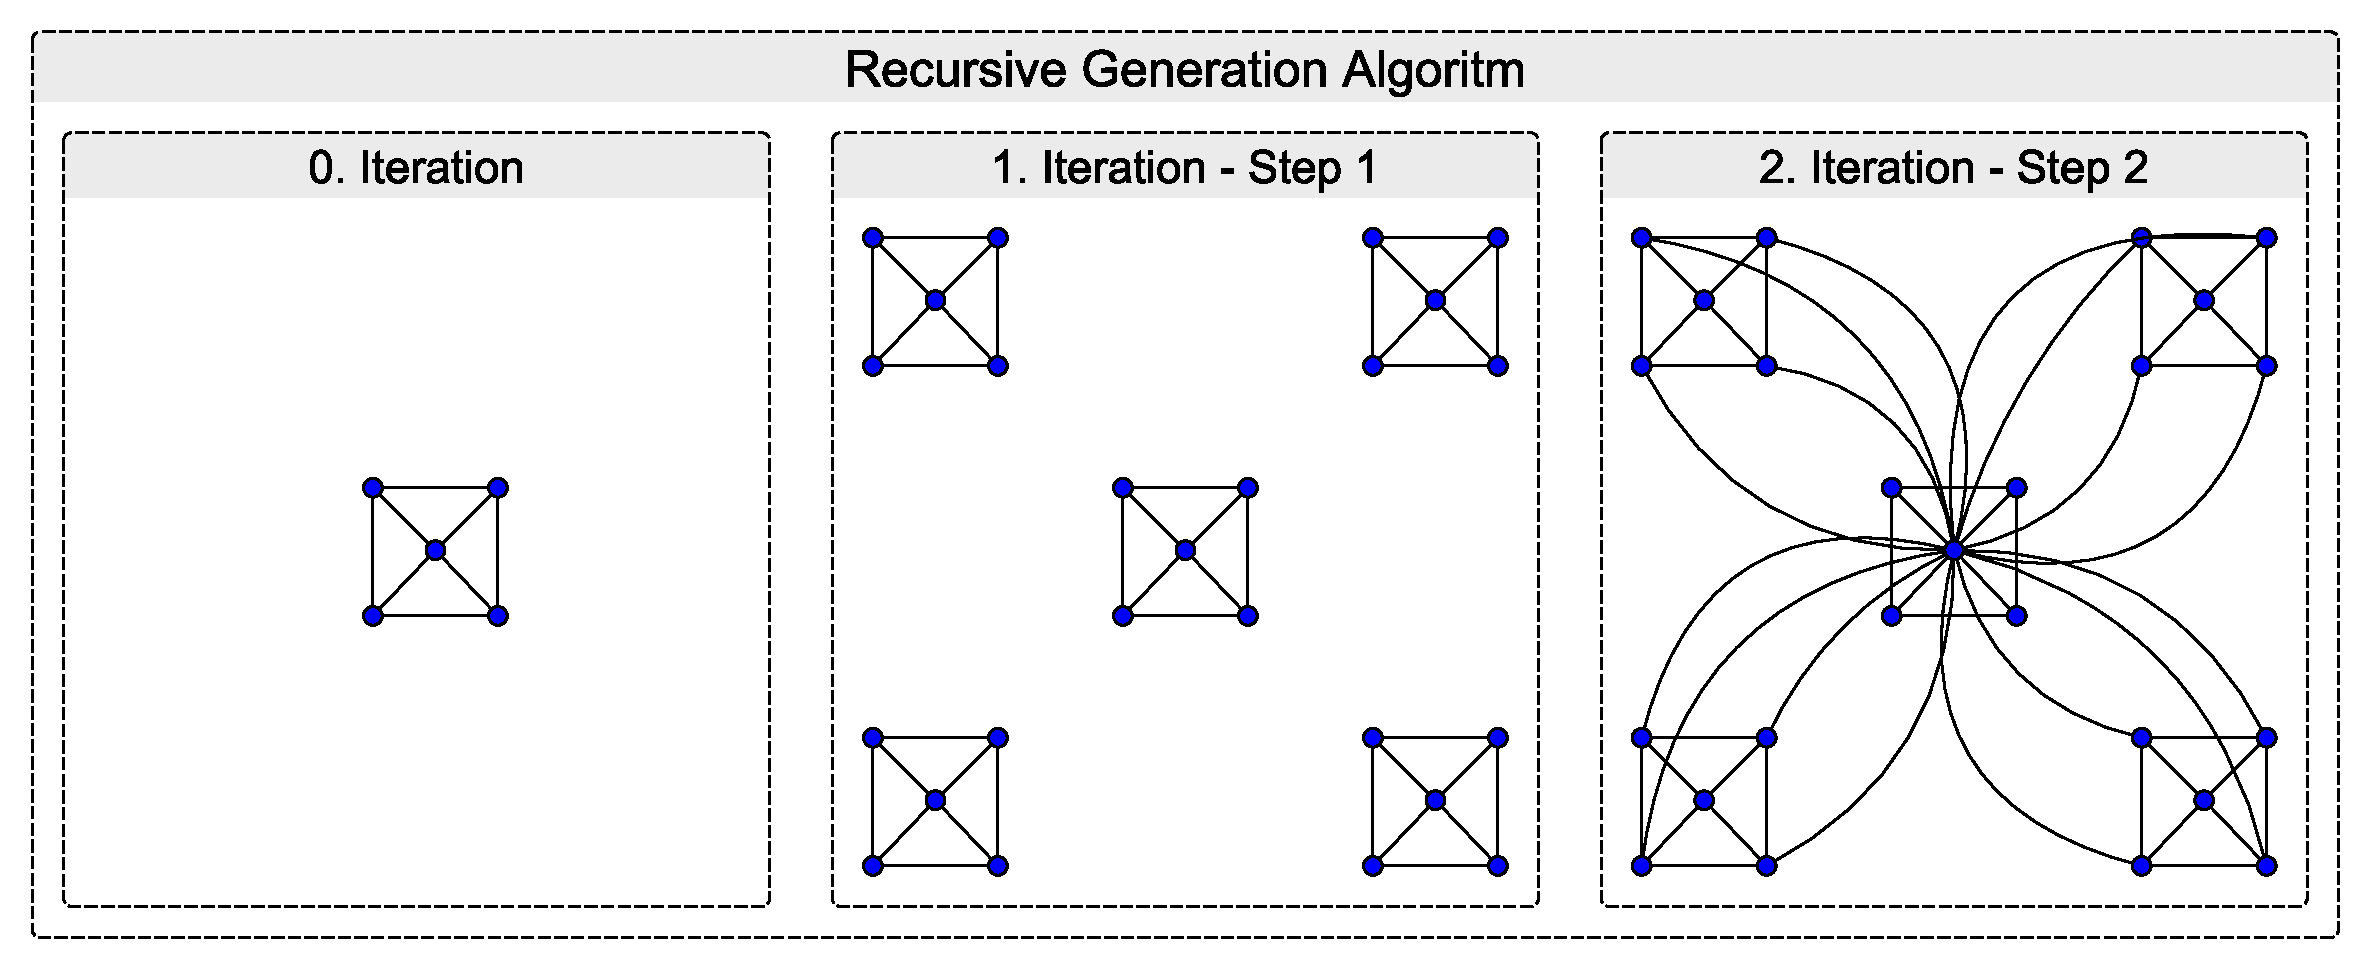
\includegraphics[width=140mm, keepaspectratio]{figures/hierarchical_generation.pdf}
	\caption{The first iteration in the recursive generation algorithm of the hierarchical network.}
	\label{fig:hierarchical_generation}
\end{figure}
